\documentclass{article}
\usepackage[paperwidth=280mm,paperheight=157.5mm,margin=16mm]{geometry}
\usepackage{fontspec}
\setmainfont{Arial}
\usepackage{graphicx}
\usepackage{xcolor}
\definecolor{navy}{HTML}{173752}
\pagestyle{empty}
\setlength{\parindent}{0pt}
\setlength{\parskip}{5mm}
\newcommand{\slide}[1]{\clearpage\color{navy}\fontsize{29}{34}\selectfont\textbf{#1}\par\color{black}\fontsize{19}{25}\selectfont}
\begin{document}
\color{navy}\fontsize{34}{41}\selectfont\textbf{Vision Transformer và ResNet\\trên CIFAR-10}\par
\color{black}\fontsize{23}{30}\selectfont
Ảnh hưởng của lượng dữ liệu huấn luyện

Lan Anh · Hiền · Minh

Bản đọc chéo nội bộ tuần 4

\slide{Dữ liệu dùng chung giữa hai mô hình}
45.000 ảnh train · 5.000 validation · 10.000 test giữ riêng

10\% = 4.500 ảnh\quad 50\% = 22.500 ảnh\quad 100\% = 45.000 ảnh

Tập con phân tầng và lồng nhau. ViT và ResNet dùng cùng manifest trong mỗi cặp seed.

Ba cặp (split, train)\quad (2026,42), (2027,43), (2028,44).

\slide{ViT tự cài có 274.282 tham số}
Ảnh 32×32 → 64 patch 4×4 → thêm CLS token

Embedding 96 chiều và positional embedding học được.

Bốn encoder block, bốn attention head, MLP ratio 1,5.

CLS → LayerNorm → Linear → logits 10 lớp.

Ablation bỏ positional embedding còn 268.042 tham số.

\slide{ResNet có 272.474 tham số}
Stem 3×3 → ba stage residual → average pooling → Linear.

Width 16, kênh 16/32/64, ba basic block mỗi stage.

Projection shortcut khi đổi shape. Khởi tạo từ đầu.

Chênh lệch số tham số với ViT khoảng 0,66\%.

\slide{100 epoch và một quy tắc chọn checkpoint}
Batch 128, cosine annealing theo epoch.

ViT dùng AdamW, LR 0,0003, weight decay 0,05.

ResNet dùng SGD, LR 0,05, momentum 0,9, weight decay 0,0005.

Chọn validation accuracy cao nhất; hòa điểm giữ epoch sớm hơn.

Mỗi tỷ lệ có 3.600 / 17.600 / 35.200 bước cập nhật.

\slide{Accuracy tăng theo lượng dữ liệu}
\begin{minipage}{0.62\linewidth}
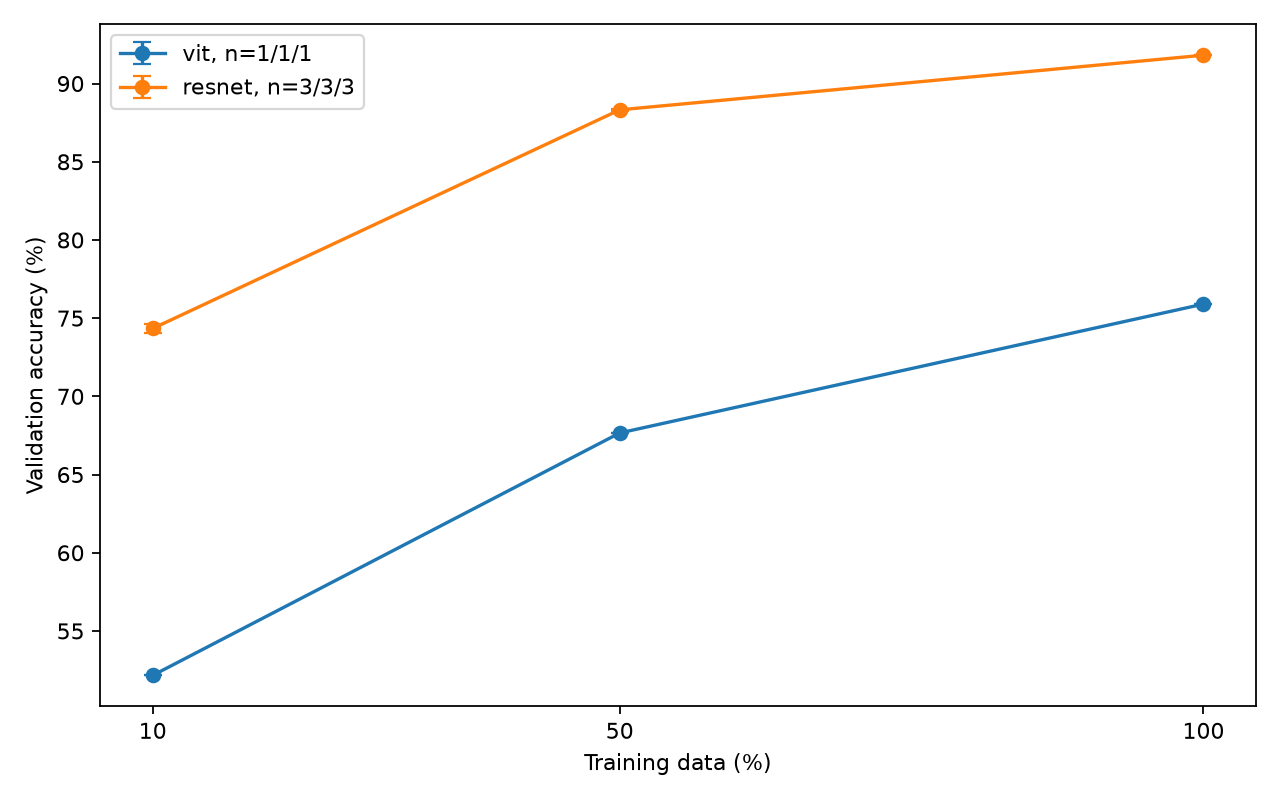
\includegraphics[width=\linewidth,height=86mm,keepaspectratio]{../results/hien_week4/validation_scaling.png}
\end{minipage}\hfill
\begin{minipage}{0.34\linewidth}
\fontsize{18}{24}\selectfont
ResNet có ba seed với log nhất quán.

ViT hiện giữ seed 42 trong bảng kiểm tra này.

Sáu log ViT bổ sung cần xác minh.
\end{minipage}

\slide{Các log bổ sung cần kiểm tra lại}
Ví dụ ViT 10\%, seed 43, epoch 1 ghi validation accuracy 0,2647.

Trên 5.000 ảnh, giá trị đó tương ứng 1.323,5 ảnh đúng.

Epoch 100 ghi thời gian train âm. Log ablation cũng có accuracy không khớp số ảnh đúng nguyên.

Cần nhận log/checkpoint gốc, đối chiếu và cập nhật bảng.

\slide{Attention validation từ bộ P0}
\begin{minipage}{0.45\linewidth}
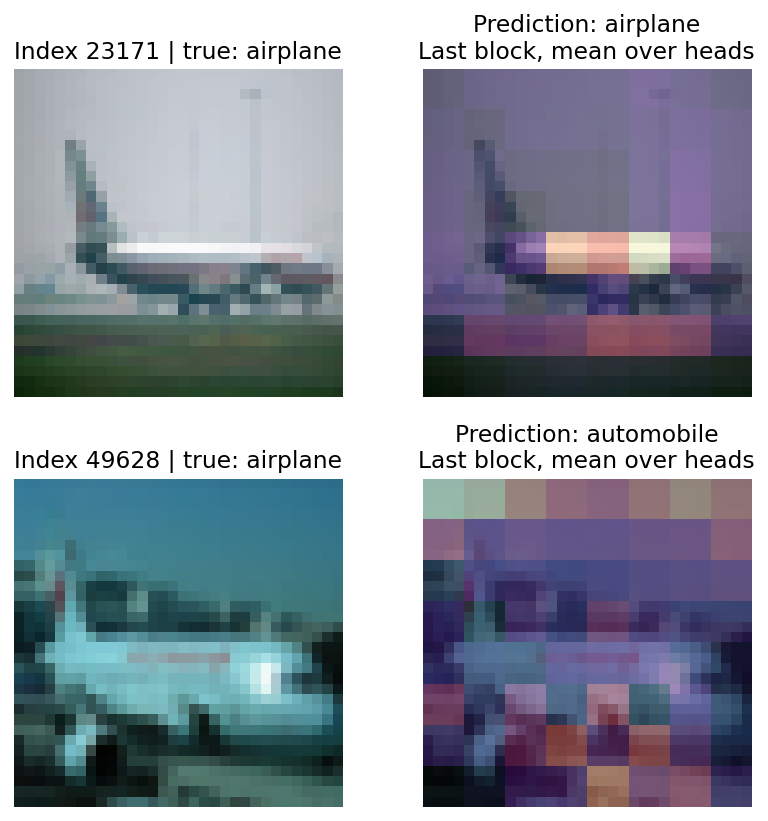
\includegraphics[width=\linewidth,height=87mm,keepaspectratio]{../results/team_week2/visualizations/5_vit_0.50_attention.png}
\end{minipage}\hfill
\begin{minipage}{0.5\linewidth}
\fontsize{18}{25}\selectfont
Ảnh đúng/sai đầu tiên theo manifest, ViT 50\%, seed 42.

CLS → patch, block cuối, trung bình bốn head; lưới 8×8.

Hình do máy GPU Minh tạo. Bộ ảnh đa lớp cố định và ghép lỗi cần checkpoint local.
\end{minipage}

\slide{Bộ tái lập và đánh giá cuối}
Một lệnh sinh lại audit, bảng từng seed, mean/SD và data scaling.

Danh sách checkpoint giữ run, seed, best validation và SHA-256.

Đánh giá test cần đủ checkpoint/config và xử lý log lỗi.

Demo ảnh 32×32 → nhãn và xác suất; attention có công cụ riêng.

\slide{Giới hạn và công việc còn lại}
Recipe của hai kiến trúc khác nhau. Tăng dữ liệu cũng tăng bước cập nhật.

ResNet validation trung bình 74,34 / 88,32 / 91,81\%.

Nhận gói checkpoint, xác minh ViT/ablation, hoàn thiện thống kê và phân tích lỗi.

Nhóm đọc duyệt số liệu, điền thông tin thành viên, khóa lựa chọn trước test cuối.
\end{document}
